\documentclass[10pt, letterpaper]{article}
        \usepackage[utf8]{inputenc}
        \usepackage[margin=1in]{geometry}
        \usepackage{fancyhdr}
        \usepackage{titling}
        \usepackage{enumitem}
        \usepackage{mathtools}
        \usepackage{amssymb}
        \usepackage{xfrac}
        \usepackage{booktabs}
        \usepackage{graphicx}
        \usepackage{wrapfig, blindtext}
        \usepackage{hyperref}
        \usepackage{enumerate}
        \usepackage{multicol}

        
        \setlength{\parindent}{0pt}

\title{Journal 2}
        \author{Sudhan Chitgopkar}
        \date{\today}
        
        % headers -- no need to change
        \pagestyle{fancy}
        \fancyhf{}
        \lhead{Cinco de Mayo}
        \chead{UGAMUNC XXVII}
        \rhead{\thedate}

\begin{document}

Dear Delegates, \\

We are so happy to welcome you to the 27th annual Model United Nations
conference here at the University of Georgia! Things are going to be a
little different this year of course, but we still hope that your
involvement in the conference is going to be a rewarding and great
learning experience. This is an opportunity to debate with like-minded
individuals about specific policy initiatives, learn about the time
period of this committee, and work on your own skills that pertain to
public speaking and writing! In La Batalla de Puebla, La Historia de
Cinco de Mayo at UGAMUNC, you'll be delving deeper into the past and
learning a bit more about the history of what happened on this historic
day in México. \\

Your first crisis director is Sudhan Chitgopkar
(\texttt{\href{mailto:sudhanchitgopkar@uga.edu}{{sudhanchitgopkar@uga.edu}}}). He is a second-year Computer Science and International Affairs double major at UGA. Sudhan loves working with organizations that are making a difference and is currently the outreach director for UGA MUN! Feel free to connect with Sudhan \href{http://follow.sudhanchitgopkar.com}{\nolinkurl{here}}! \\

Your second crisis director, Alexa Hernandez
(\texttt{\href{mailto:agh56717@uga.edu}{{agh56717@uga.edu}}}), is a
third-year student studying Political Science and International Affairs
here at the University, while pursuing a certificate in Public Affairs.
She has been involved with Model United Nations, both in college and in
high school, and currently serves as one of the Head Delegates for the
team. Alexa is interested in going to law school once she graduates and
hopes to be an influential leader on the world stage! \\

Additionally, Nathan Yu
(\texttt{\href{mailto:nathanyu98@uga.edu}{{nathanyu98@uga.edu}}}) will
be your chair. He is a third-year Marketing and International Business
major at UGA, with an immense passion for linguistics/learning languages
that has led him to pursue minors in German and Spanish. Model United
Nations has been a valuable learning experience for Nathan so far and
has allowed him to meet many talented peers! Nathan's primary goal is to
become a high-functioning polyglot through his current studies in
German, Spanish, Korean, Portuguese, French, along with working
knowledge in Russian, Italian, and Dutch. \\

Your co-chair for the weekend will be Sophia Kwan (\texttt{\href{mailto:sophiakwan@uga.edu}{(sophiakwan@uga.edu)}}).
She is a first-year Advertising major with minors in Spanish and Business. Sophia has been involved in Model UN throughout high school and is excited to be part of the UGA team. She enjoys volunteering with the Guide Dog Foundation and is training to be a puppy raiser. In her free time, Sophia enjoys spending time with her friends, photography, trying new coffee shops, and traveling to other countries! \\

We know that you'll all do a fantastic job bringing your role to life in
conference. If you have any questions please don't hesitate to contact
us. Welcome to UGAMUNC XXVII! \\

Sincerely,\\
Alexa Hernandez and Sudhan Chitgopkar \\
Crisis Directors, La Batalla de Puebla, La Historia de Cinco de Mayo

\newpage
\tableofcontents
\newpage

\section{{Rules and Procedure:}}
\subsection{General Rules}
While other delegates at UGAMUNC may be placed in traditional General
Assembly-style Model United Nations committees, La Batalla de Puebla, La
Historia de Cinco de Mayo committee at UGAMUNC will run as a crisis
committee. While you should still familiarize yourself with the UGAMUNC
Rules and Procedure document to brush up on parliamentary procedure,
this committee will vary from the typical format. Please familiarize
yourself with the following rules specific to this committee, and once
again, if you have any questions, feel free to reach out to Sudhan or Alexa
at
(\texttt{\href{mailto:sudhanchitgopcar@uga.edu}{{sudhanchitgopkar@uga.edu}}})
or (\texttt{\href{mailto:agh56717@uga.edu}{{agh56717@uga.edu}}}).

\begin{enumerate}
\def\labelenumi{\arabic{enumi}.}
\item
  
  \textbf{This committee is loosely based on the La Batalla de Puebla.}
  This is the general topic of our crisis committee, and as members of
  the acting countries involved or related individuals, this will be the
  focus of much of the conversation for the weekend. However, you are
  more than welcome to focus on related issues of the times or alter the
  path of history forever.
  
\end{enumerate}

\begin{enumerate}
\def\labelenumi{\arabic{enumi}.}
\setcounter{enumi}{1}
\item
  
  \textbf{While this is a historical committee, you have the freedom to
  alter history.} This committee is to be set in the city of Puebla and
  the surrounding area in the year 1862, where México is still reeling
  from the liberals being able to take back México City the previous
  year. While members of this body should consider any events that took
  place prior to May 3rd, 1862, as historical facts in this committee,
  any events that occurred after that date will not automatically occur.
  Characters in this body have a chance to rewrite fate in the manner
  they choose.
  
\end{enumerate}

\begin{enumerate}
\def\labelenumi{\arabic{enumi}.}
\setcounter{enumi}{2}
\item
  
  \textbf{Utilize crisis notes to accomplish your goals in committee and
  craft your crisis arc.} While the main method of negotiation in a
  typical General Assembly-style committee stems from typical speaking
  time work in committee, in a crisis committee, much of the work you do
  will be on your own through crisis notes. These are letters that your
  character will write to crisis, a body outside of the committee room,
  to accomplish something without the committee's knowledge. A good
  crisis note not only explains, in detail, what to do, but it also
  explains very specifically how to do it. These notes will be addressed
  to a fictional person that has some relation to your character.
  ``Crisis'' (UGAMUNC staff and your crisis director) will answer these
  notes as if they were this fictional person, responding as that person
  would under the circumstances from the context you set out. Only
  address a note to crisis if you have a question about the way the
  committee is going. There are many fantastic resources that better
  explain crisis notes in detail, but a starting point can be found
  here:
  \href{http://bestdelegate.com/the-three-crisis-notes-to-send-at-the-beginning-of-any-model-un-crisis-committee/}{{http://bestdelegate.com/the-three-crisis-notes-to-send-at-the-beginning-of-any-model-un-crisis-committee/}}
  
\end{enumerate}

\begin{enumerate}
\def\labelenumi{\arabic{enumi}.}
\setcounter{enumi}{3}
\item
  
  \textbf{Because this is a crisis-style committee, write directives,
  not resolutions.} Although they are very similar, directives are the
  typical formal paper written in a crisis committee, not resolutions.
  Directives are less formal, are normally titled, and are generally
  more straightforward. They are intended to utilize the powers present
  in the committee to quickly address the crisis at hand or any related
  issues.
  
\end{enumerate}

\begin{enumerate}
\def\labelenumi{\arabic{enumi}.}
\setcounter{enumi}{4}
\item
  
  \textbf{Represent your understanding of your character.} This is a
  historical crisis committee, meaning that a few of these people
  actually existed and were somehow involved in la Batalla de Puebla.
  Use this to your advantage; do some research! Each character is
  unique, and therefore has unique goals and relationships among members
  of the committee. That said, be sure to represent your character's
  beliefs and not simply your own. While you may not be prepared for the
  updates which crisis will present to you, you can at least understand
  the character you have been assigned and react to crisis in the way
  they would.
  
\end{enumerate}

\begin{enumerate}
\def\labelenumi{\arabic{enumi}.}
\setcounter{enumi}{5}
\item
  
  \textbf{Be as historically accurate as possible.} Because this is a
  historical committee, it is expected that all delegates will act in a
  manner that suits the time period. We'd like you to understand the
  location and time period in which the committee is set, and this will
  require doing prior research. This also means that some convenient
  technologies may not have been invented yet, and are therefore not
  available in committee. For example, emailing a friend via a crisis
  note would be impossible, but sending them a letter via horseback
  would be fine.
  
\end{enumerate}

\begin{enumerate}
\def\labelenumi{\arabic{enumi}.}
\setcounter{enumi}{6}
\item
  
  \textbf{This committee is English only.} Even if you can speak
  Spanish, there will be no advantage given to any delegate who chooses
  to write crisis notes or give speeches in Spanish. While we certainly
  respect historical and cultural accuracy, we don't want to exclude
  other delegates in committee who may not speak Spanish (including your
  chairs).
  
\item
  
  \textbf{All position papers for this committee are due on February 7
  by 11:59pm.} Please submit these position papers directly to the both
  of us at
  (\href{mailto:sudhanchitgopkar@uga.edu}{{sudhanchitgopkar@uga.edu}})
  and (\href{mailto:agh56717@uga.edu}{{agh56717@uga.edu}}). A
  position paper is essentially a short letter outlining your
  character's position on the crisis at hand and your individual plans
  to accomplish those plans. We expect these papers to be around one (1)
  double-spaced page in length. We've attached some resources below to
  help you get started. Happy writing!
  
\end{enumerate}

\subsection{Position Paper Resources}
\begin {itemize}
\item
Best Delegate:
\texttt{\href{https://bestdelegate.com/how-to-write-a-winning-position-paper/}{{https://bestdelegate.com/how-to-write-a-winning-position-paper/}}}
\item
NMUN:
\texttt{\href{https://www.nmun.org/assets/documents/NMUNPPGuide.pdf}{{https://www.nmun.org/assets/documents/NMUNPPGuide.pdf}}}
\item
AMUN example papers:
\texttt{\href{https://www.amun.org/sample-paper-1/}{{https://www.amun.org/sample-paper-1/}}}
\end{itemize}
\newpage
\section{{Background of Committee}}

\subsection{The War of Reform}

\begin{wrapfigure} {l} {0pt}
\centering
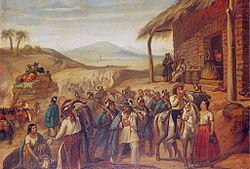
\includegraphics[width=2.61111in,height=1.76389in]{image8.jpg}
\caption{Soldiers of the Reformation, 1858}
\end{wrapfigure}

The War of Reform was a three-year-long, politically-founded civil war
in México that would later set the stage for the election of president
Benito Juárez and the events of May 5th, 1862. This war was fought
primarily between the liberal and conservative political parties of
México as a result of their separate beliefs regarding a set of new laws
passed by the liberal individuals in the government. The liberals
believed in increased separation of church and state in México, and they
wanted a smaller military overall. As a whole, liberals saw the Catholic
Church and the army to be antiquated institutions which had little place
in México. The conservative politicians in Mexico had a different take,
prioritizing strong central governments with traditional roles for the
Catholic Church and military. Conservatives also largely aligned with
the idea of maintaining racial hierarchies in México with the minority
merchant elites being superior to the majority mixed-race and indigenous
population.\footnote{Hamnett, Brian. ``Mexican Conservatives, Clericals,
  and Soldiers: the `Traitor' Tomás Mejía through Reform and Empire,
  1855--1867.'' \emph{Bulletin of Latin American Research} 20, no. 2
  (2001): 187--209. https://doi.org/10.1111/1470-9856.00010.} \\

The war began as a result of the Constitution of 1857 being passed by
the liberals as it provided a constitutional basis for them to implement
a series of laws that defunded and separated out much of the Catholic
Church from the central government. The Conservatives, outraged by the
new constitution, passed the Plan of Tacubaya in a closed Congress,
which allowed them to oust the Liberals from México City, forcing them
to reallocate to Veracruz.\footnote{Hamnett, Brian. ``The Comonfort
  Presidency, 1855-1857.'' \emph{Bulletin of Latin American Research}
  15, no. 1 (1996): 81--100.
  https://doi.org/10.1111/j.1470-9856.1996.tb00023.x.}\\
  

From there, the real fighting began. Some states decided to side with
Félix Zuloaga, who was the ``leader'' of the conservatives. Others
fought alongside Benito Juárez, leader of the liberals. Few stayed
neutral. \\

While the liberals suffered heavy casualties and lost the vast majority
of their early battles against the Conservatives, they were always able
to ward off take-over attempts of Veracruz, the liberal capital and
stronghold. Things seemed relatively bleak for the liberals. By a stroke
of luck, though, the liberals went on to win repeated battles until the
conservatives surrendered in December of 1860. \\



On January 15, 1858, Benito Pablo Juárez Garcia, President of the
Supreme Court of Justice and Vice President, assumed presidency
following Ignacio Comonfort fleeing to the United States. Comonfort was
the previous, unpopular President of México: he fled to the United
States because he was unsupported by both parties and hated by the
public. Despite the order of succession, the conservative forces did not
acknowledge his presidency and named Felix Maria Zuloga as the interim
president in México City.\footnote{Coerver, Don M., Suzanne B. Pasztor,
  and Robert M. Buffington. 2004. \emph{México: An Encyclopedia of
  Contemporary Culture and History}. Santa Barbara, California:
  ABC-CLIO.\href{https://books.google.com/books?id=YSred4NyOKoC\&printsec=frontcover\#v=onepage\&q\&f=true}{{https://books.google.com/books?id=YSred4NyOKoC\&printsec=frontcover\#v=onepage\&q\&f=true}}}
The struggle for power between the conservatives and liberals continued
throughout Juárez's interim presidency. Juárez established a liberal
government in Queretaro, later moving it to Veracruz. He issued various
decrees known as the Reform Laws which included separating church and
state, nationalization of church property, and establishing a civil
registry for births, marriages, and deaths. The Reform Laws would limit
the power of the Catholic Church guaranteeing freedom of religion, they
were later approved by congress in May of 1861.\footnote{Lee, Stacey.
  2003. \emph{México and the United States}. Tarrytown, New York:
  Marshall Cavendish.
  https://books.google.com/books?id=DSzyMGh8pNwC\&printsec=frontcover\&source=gbs\_ge\_summary\_r\&cad=0\#v=onepage\&q\&f=false.} \\

\subsection{The Election of Benito Juárez}
\begin{wrapfigure} {r} {0pt}
\centering
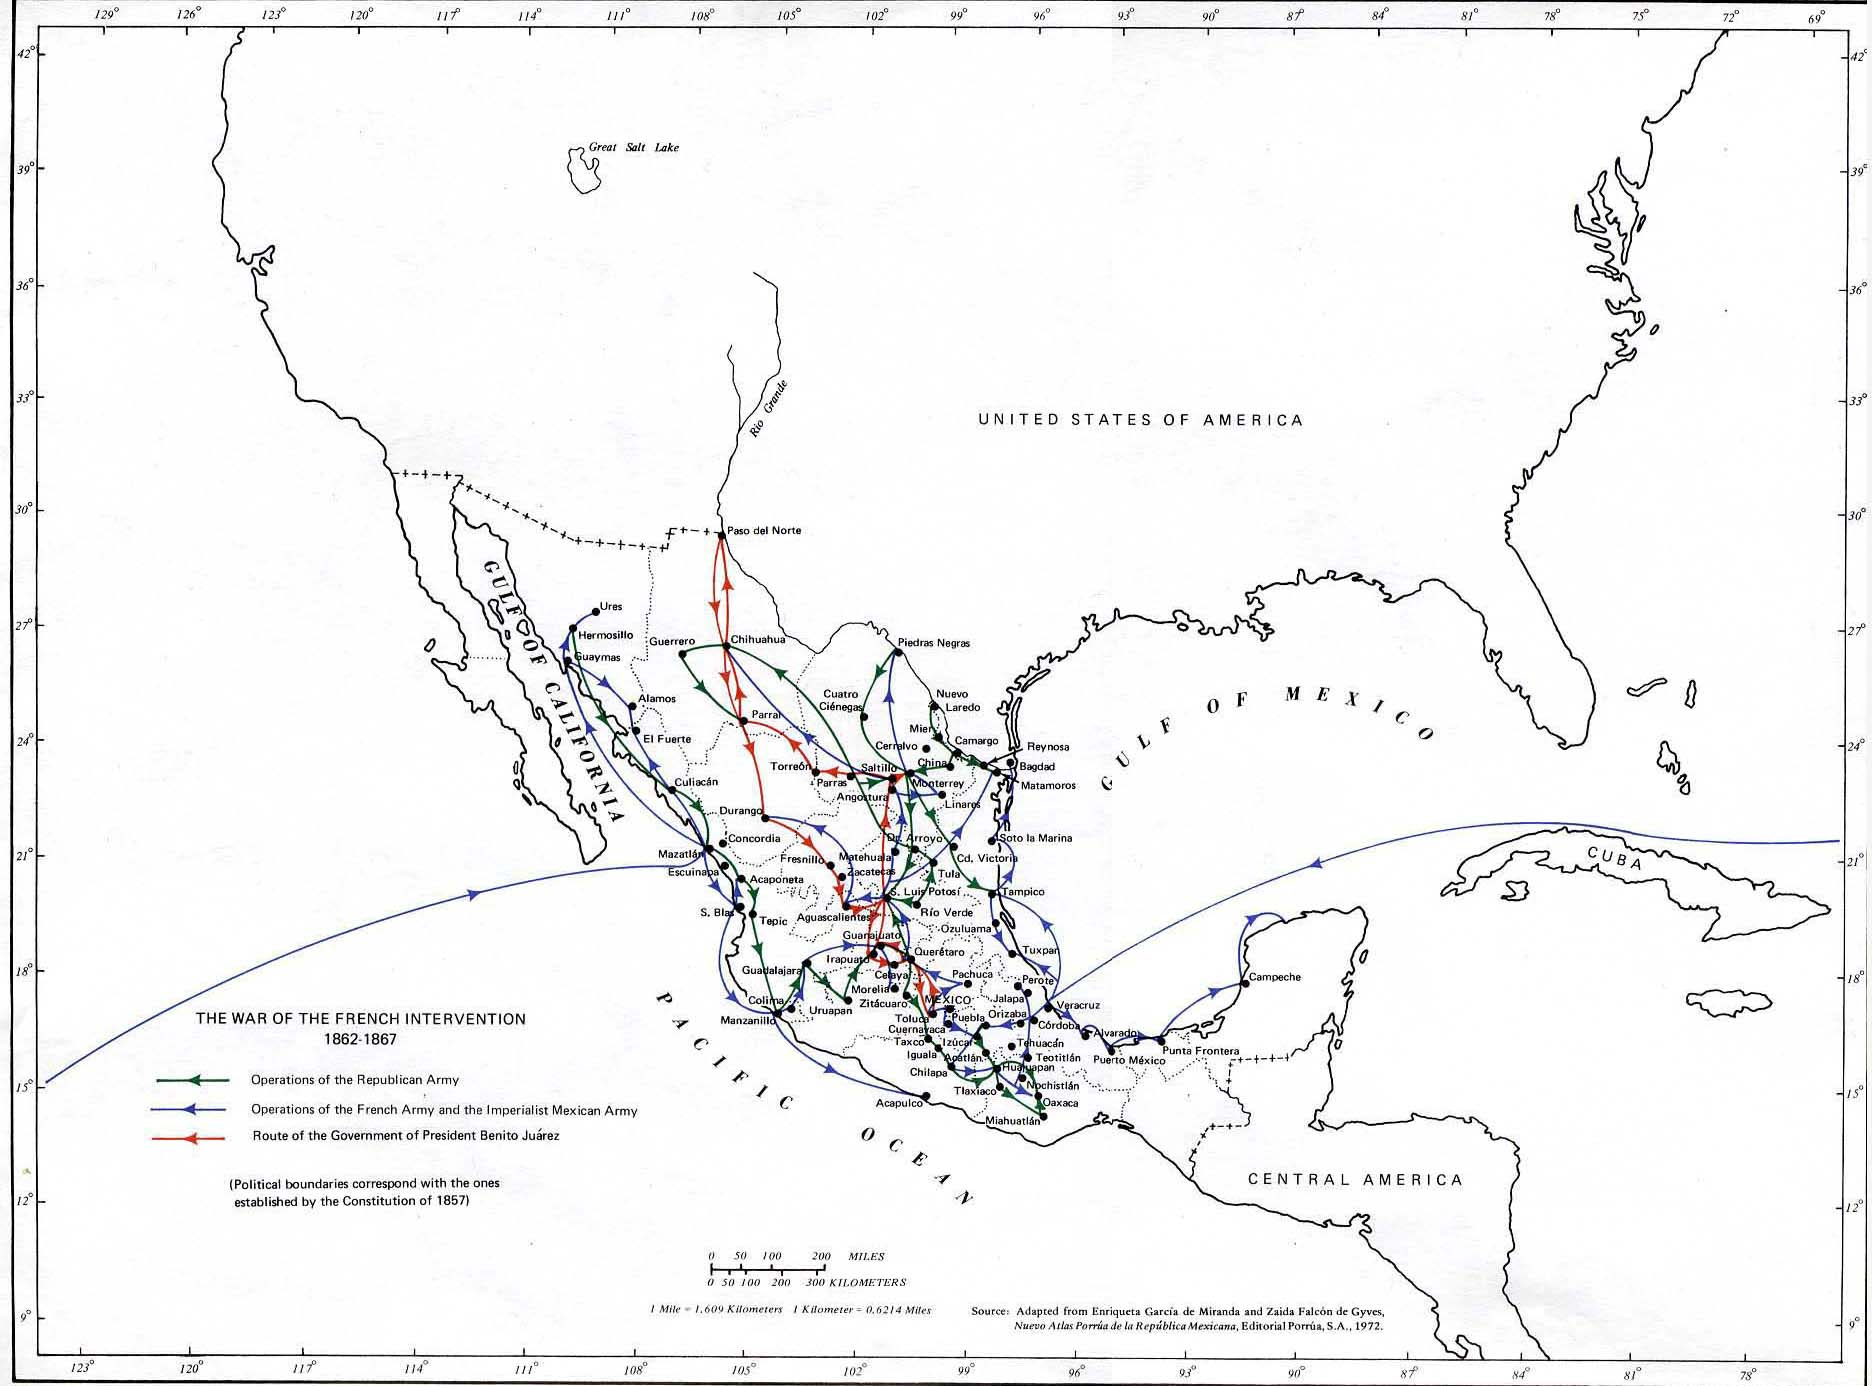
\includegraphics[width=3.06771in,height=2.2762in]{image5.png}
\caption{Map of French Intervention Routes}
\end{wrapfigure}
Following the war in 1861, Juárez called for a referendum, which
formally elected him as president: giving him control of México City. He
entered office facing a crippled economy and a heavily divided country.
Additionally, he faced strong criticism within his own party. A
resolution in the lower house of Congress called for his resignation,
and it was defeated by only one vote. \\

The treasury was exhausted following the war, and there was little
trade. Foreign powers such as England, France, and Spain were demanding
repayment of their loans, which México did not have the funds to do
so.\footnote{Library of Congress. 1997. ``México: A Country Study.''
  Fourth Edition:435-436.} This caused a lot of issues within México, as
the government was trying its best to stay stable with pressures from
outside powers and an economy that was in shambles. Additionally, México
was unable to turn to the United States for financial assistance, as
they were entering their own civil war. Tensions were mounting between
these two countries, as the annexation of Texas happened a few years
prior in 1845. This annexation led to the Mexican-American war, which
began in 1846, and lasted two years. While this conflict started over a
disagreement of México's true northern border, the war allowed for the
United States to exert power over the newly independent México. Due to
this turmoil, Juárez declared a two year suspension on foreign debt
repayments, furthering the tensions at home and abroad. \\

\subsection{The Stirrings of War (Part I)}

Angered by Juárez's refusal to make good upon foreign debt interest
payments, a tripartite alliance was formed by France, Spain, and the
United Kingdom with the sole intention of invading México as a mechanism
to enforce interest payments. It is important to note that the United
Kingdom specifically opposed using this as an attempt to incite regime
change in México, fearing encroaching on American influence in the
region. Spain and France disagreed, noting that if the Mexicans wanted
regime change, the European powers should help them bring that about.
While these differences were put aside during the signing of the
tripartite alliance, they still existed as the invasion of México would
begin. For Spain and the United Kingdom, this was simply a means to
coerce back payments on interest. The French, however, had other plans. \\

\subsection{France under Napoleon III}

Napoleon III had a successful, if controversial, time as ruler of
France. He began as the elected President of France, eligible for a
single, four year term.\footnote{Delage, Irène, and Nebiha Guiga.
  ``Napoleon III, Emperor of the French (1808-1873).'' napoleon.org.
  Fondation Napoléon 2020, 2016.
  https://www.napoleon.org/en/young-historians/napodoc/napoleon-iii-emperor-of-the-french-1808-1873/.}
The French Constitution, as a means of preventing abuse of power, capped
the maximum term limit for presidents at this aforementioned one,
four-year term. This wasn't enough for Napoleon III, and he spent the
third year of his four years in office attempting to pass an amendment
that would allow him a second term. This amendment failed due to
concerns about Napoleon's unchecked power should he receive a second
term. As a result, Napoleon spent time gaining as much popularity as
possible in France and ended his final year of presidency by declaring
himself Emperor of
France. \\

 As a result of his emperorship becoming initially contingent upon his
popularity, Napoleon III took significant steps to center his domestic
policy around maintaining popularity in France. To that end, he promoted
construction and industry projects, promised better conditions for the
poor, and specifically provided many benefits to workers in the industry
sector. \\

Internationally, Napoleon III was adamant upon restoring the empire of
France. As such, his imperialist tendencies had few bounds. The
establishment of the tripartite alliance and the inability for México to
pay back foreign debt interests opened the door for Napoleon III to
begin military conquest in México. Such conquest was driven by two
factors: (1) a general ability to advance French influence across all
corners of the globe and (2) the ability to counterbalance the United
States which was, at this time, moving into the first tides of civil
war: threatening the influence that France had in Europe. \\

\subsection{The Stirrings of War (Part II)}

On November 11th, 1861, Napoleon III instructed his vice admiral to not
only capture the ports of México but to hold them until the debt issues
had been resolved. It is unclear whether the other members of the
tripartite alliance knew about this, but it is unlikely. Alongside the
rest of their tripartite alliance, France began their invasion of
México. Spanish forces were the first to land in the city of Velacruz on
December 8th, 1861. These some 6,000 troops gave the governor of
Veracruz a final opportunity to surrender, which was ignored. Three days
after this surrender opportunity, the Spanish conquered Velacruz. In
doing so, they violated the tripartite agreement, which stipulated that
all actions would be conducted by all three countries in the
agreement.\footnote{``The Cinco De Mayo and French Imperialism.''
  napoleon.org. Fondation Napoléon 2020. Accessed October 20, 2020.
  https://www.napoleon.org/histoire-des-2-empires/articles/the-cinco-de-mayo-and-french-imperialism/.} \\

\begin{wrapfigure} {r} {0pt}
\centering
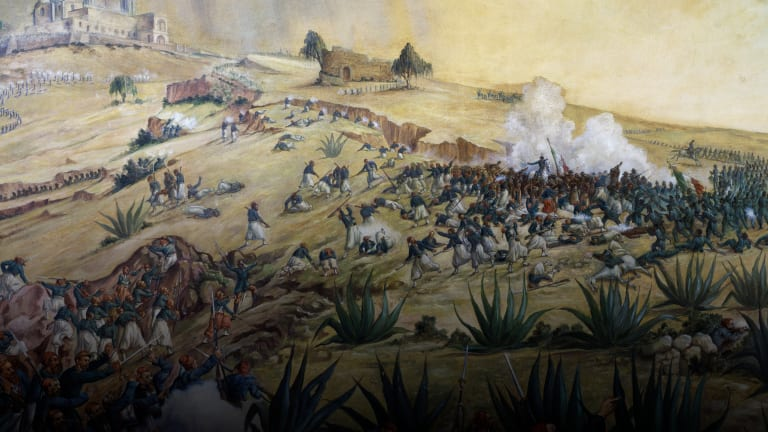
\includegraphics[scale = 0.35]{image1.jpg} 
\caption{Mexican Army Repels French Forces}
\end{wrapfigure} 

Shortly after this, French and British forces landed in México, in close
proximity to the Spanish forces at Veracruz. At this point, one final
ultimatum was given out by the tripartite alliance to México. This
ultimatum demanded twelve million francs from the Mexican government as
repayment of all debts and debt interests accrued by México. México refused this ultimatum, so on April of 1862, the first battles began. France officially declares war on México on April 20th, after a military skirmish between French and Mexican forces a day earlier resulted in casualties on the Mexican side. Skirmishes and small wars keep occurring through April, getting larger and larger with each passing day until the 28th when the French army reaches Puebla. The French have 5,000 troops, 10,000 fewer than they were promised. As such, they were vastly outnumbered by the 12,000 Mexican troops holding Puebla. \\

As such, the Battle of Puebla began. \\

\newpage
\section{{Starting Scenario}}

\textit{May 3rd, 1862, the City of Puebla in East-Central México:} \\

Tensions have begun to rise as the quest for new land continues to bring
the world together, and drive it further apart. As a newly independent
country from Spain, México is in the process of fighting for legitimacy
on the world stage, and pushing for a solid authority figure to lead the
country further away from the shadow of Spanish rule. With the continued
rule of weak and bankrupt governments, a recent crippling civil war, as
well as the unwise economic decisions made by said governments, México
is struggling to stay footed as a republic. Additionally, pressures from
the United States over the borders of Texas have left the country more
scattered than before, with Texas formally becoming annexed by the
United States in 1836. In 1861, after the election of President Benito
Juárez, México was in a state of economic turmoil due to years of
payment mishandling and corruption within the government. Creditors
France, Spain, and the United Kingdom met in London to form an alliance
with the sole purpose of launching an invasion into México to demand
repayment. While the United Kingdom and Spain quickly withdrew from this
deal, France is continuing on the path of war against México. \\

While this is not canon, you all will be meeting in Puebla to discuss
avenues at a jointly-called peace summit. Tensions have not yet risen
past the point of no return, so it is in all of your best interests to
come to a solution that benefits all of the parties involved. \\

However, as members of these warring parties, you each have goals of
your own. The path toward peace is not going to be an easy one, and it
is pertinent that you all work together to achieve a common goal for the
sake of both France and México, as well as all other actors who may
arise as time moves on. However, this is happening during a time where
economic turmoil is not only occurring in México. The entire world is
fighting to become more prominent than their allies and adversaries.
Debts must be repaid, and in whatever way that is done, each country is
going to be expecting something at the pinnacle of debate. The group of
politicians, generals, and leaders of their respective fields in this
committee are the most prepared to undertake this challenge of what is
sure to be war if tensions do not settle. Although you each know what
your respective goals are, you are more than ready to fight to the end
for justice, and for your country. \\

While your goals in this committee may overlap, you should make it a
point to increase your overall power in committee by accumulating
friends and resources to better prepare yourself and your allies for
what is to come. Additionally, working with other committee delegates to
create a deal, or perhaps requesting aid from foreign countries in the
fight against aggressors, may be necessary. You'll have to take into
account other societal problems of the era, seeing as to the North there
is a Civil War going on, as well as pressures coming from European
powers. It is up to you to work diligently despite the state of the
world, and come up with a comprehensive solution. \emph{Al mal paso,
darle prisa.} \\

\newpage
\section{{Character Descriptions}}

\begin{enumerate}
\def\labelenumi{\arabic{enumi}.}
\item
  
  \textbf{Napoleon III, Empereur-} As the founder, first, and only
  emperor of the Second French Empire, Charles-Louis Napoleon Bonaparte
  cemented himself as one of the most important figures in the 19th
  century. He is the nephew of Napoleon I, and inherited the immense
  craving for power and dominance that his uncle had. He takes great
  pride in his mustache, and has the reputation of being protective of
  it at all times.
  
\item
  
  \textbf{Félix María Zuloaga, General -} Félix is a Conservative leader
  first, and a general second. Despite his influence within the
  Conservative party, Félix has trouble keeping a footing within the new
  government under Benito Juárez. Additionally, although he was the
  President before Juárez, he has become a political outcast. Shaken
  from the loss of power, he is looking for a new movement to follow.
  \emph{Pouvez-vous parler français?}
  
\item
  
  \textbf{General Charles de Lorencez, Chef de la force expéditionnaire
  française -} As Napoleon's favored general, Charles is an experienced
  strategist and influence on the French's battle plans. As well as
  being Napoleon's favored general, he also is in a competition against
  Napoleon for the greatest mustache in France. His newest assignment
  seems to be taking him to a country near the United States, but he
  knows that whoever they are, they better be ready for the mighty
  armies of France.
  
\item
  
  \textbf{Ignacio Zaragoza, Comandante-General} - Although Ignacio comes
  from a simple background, this does not detract from the mastermind
  that this general is. As the previous Secretary of War, Zaragoza
  understands the pressures México is under and the best ways to solve
  them. Most of the armies are loyal to him as well, seeing as he is a
  benevolent leader. He may be misguided at times, but has a heart of
  gold.
  
\item
  
  \textbf{Porfirio Díaz, Brigadier General} - As a war veteran from the
  War of Reform, Porfirio is a well-respected general throughout México
  with an adamant dislike of everything French. Since his first
  enrollment in the army as a teenager in 1846, he has moved through the
  ranks quickly. However, he did not always want to become a fighter:
  his plans to become a priest halted when recruits were needed for the
  War of Reform. He still is a deeply religious man, seeking council
  from the Pope when needed.
  
\item
  
  \textbf{Élie Frédéric Forey, Commandant-Général -} Élie is a man of
  honor, as he is very loyal to the French crown. Having served in 3 or
  so wars thus far, he is not worried about his new assignment as
  commanding general of the French expeditionary corps to México. He is
  excited for the opportunity to gain new distinctions in the French
  military, and hopes to continue climbing the ranks until he can no
  longer do so. He has heard a lot about México, and is excited to make
  some money off of its government.
  
\item
  
  \textbf{Archduke Ferdinand Maximilian -} As a highly charismatic
  Austrian, Ferdinand knows how to work a crowd; he is well educated,
  joyful, but also a little bit undisciplined. Although these traits are
  working against him, he has the opportunity to become the emperor of
  México. He turned down the first proposal to explore the beautiful
  forests of Brazil (he's a huge botany nerd), and now is working on
  behalf of the Mexicans to help in their fight against tyranny.
  
\item
  
  \textbf{Ignacio Comofort, Vigésimo Quinto Presidente de México-} After
  the ratification of the Constitution of 1857, many anti-constitutional
  forces, including General Zuloga, were not happy with their president.
  Comonfort resigned as President and fled to the United States, seeking
  asylum from México's neighbors to the North. Upon hearing about the
  trouble in his home country, he has put aside all past grievances and
  has returned to México to fight for his country again. With a war
  brewing, and past trauma holding him back, what will he do?
  
\item
  
  \textbf{Manuel Dublán, Abogado -} Brother-in-law to Benito Juárez,
  Dublán is a leading figure in Mexican politics, supporting liberal
  ideology through his law practice. He helped draft the ``Ley Juárez,''
  the first of the Reform Laws setting the stage for his brother's
  presidency. He is fearlessly loyal to his brother and México, and he
  is an aggressive litigator. Don't get into a legal argument with him!
  
\item
  
  \textbf{Miguel Negrete Novoa-} Originally part of the military under
  Comonfort's rule, he believes in conservative principles and takes
  pride in his country. With the impending French invasion, Novoa
  decided to put his country before his ideology stating ``Tengo una
  patria antes que un partido político,'' meaning ``I have a country
  before a party.'' He joins the liberal forces commanded by Ignacio
  Zaragoza and is ready to fight for his country!
  
\item
  
  \textbf{Tomás O'Horán Escudero, General-} Not to be confused with his
  father, Tomas Antonio O'Horan y Agüero, Escuerdo is a loyal fighter
  for México, participating in every battle throughout his lifetime.
  Known throughout México as the ``the Immortal of Atlixco,'' he seems
  to have a lucky streak when he fights in battle. He stands by Benito
  Juárez and the liberals, and loves his home country more than
  anything. Will his ``immortality'' hold up in what could be México's
  historic battle?
  
\item
  
  \textbf{Juan Nepomuceno Méndez, General-} Méndez once lived a simple
  life as a working-class citizen of México, but when soldiers were
  needed in the Mexican-American War, he enlisted and has not looked
  back since. He worked his way through the ranks, and now serves as a
  General. Ready to defend his country from the French, he stands by his
  close friend, a fellow liberal, Portfolio Diaz.
  
\item
  
  \textbf{Francisco Lamadrid, General -} Lamadrid has loved México ever
  since he was a young child. Rumor has it, his first words were ``amo
  México'' (though this can't be confirmed). A good friend to Juárez,
  Lamadrid has worked his way up through the army ranks, and now sits as
  General with an ``in'' to the President. He has a well-founded
  political opinion on everything in the world and is widely considered
  to be one of the best academics in his community. On the side, Carlos
  has an affinity for chess, something that may give him an upper hand
  in battle-planning.
  
\item
  
  \textbf{Jean Danjou, Capitaine -} As an expert military man and
  distinguished graduate of France's premiere military academy, Jean has
  a reputation that precedes him. His recent call to action was to
  command a unit of mercenaries and degenerates: individuals who respect
  and obey Jean's orders despite their instincts to rebel. Many years
  ago, his left hand was lost during a battle, and now he sports a fake
  wooden hand that he uses as a personal club. Don't get too close when
  he's in a bad mood.
  
\item
  
  \textbf{John Waigne -} As a gun-toting, horse-riding renegade from the
  US, John Waigne cares very little about the politics behind the la
  Batalla de Puebla. He's an expert marksman and a charismatic (if
  sometimes apathetic) leader that is renowned for his dueling and
  fighting abilities. He's always saving the world, chasing the girls,
  and just happened to get caught up in the middle of this standoff.
  
\item
  
  \textbf{Henry Seward, Nomad/Salesman-} Seward, an American, comes from
  an eccentric French heritage: his grandfather, a French noble, decided
  to give up his riches in pursuit of the fountain of youth. His journey
  took him to the United States where he became an inventor and
  developed a miraculous snake oil medicine, as well as a popular line
  of weaponry. These inventions earned Seward's grandfather the millions
  he had left behind in France. Armed with his grandfather's inheritance
  and an inventive mind of his own, Seward set off in pursuit of the
  fountain of youth that his grandfather was never able to find. His
  journeys landed him in Puebla amidst the stirrings of war.
  
\item
  
  \textbf{Javier Philip II-} As a member of the French army, Javier
  Philip II was excited to finally step into battle and expand his
  country's empire as much as possible. He comes from a family of means
  and received a proper education during his early years: he's a master
  swordsman! Despite being issued a musket by the French, he prefers to
  do battle with a sword that he created himself (which he
  affectionately calls a ``Hattori Hanzō''). He despises the
  hack-and-slash nature of war, preferring to be a smart, cunning, and
  stealthy assassin instead. Enchanted by Mexican culture and bored of
  French imperialism, he surrendered himself to Benito Juárez, who saw
  him fit to be an important part of the Mexican army.
  
\item
  
  \textbf{Emile Marty-} Despite being one of the strongest, most brutish
  fighters for the French, Emile was forced to surrender himself to the
  Mexican army during one of the early skirmishes. He was kept as a
  prisoner by the Mexican army, but escaped his cell and slipped out
  under the cover of darkness. During his time as a prisoner, Marty
  learned a lot about the plans of the Mexican army and their battle
  structure. His information could be of great use to the French army,
  but he feels somewhat betrayed by their lack of an attempt to save
  him. Is this enough to make him sway sides? For now, though, he's just
  an angry, strong, and vengeful man with a loyalty only to himself.
  
\item
  
  \textbf{Maria Fermina Rivera, Veterana de guerra -} Coming from a
  background of insurgence fighting in the Mexican War of Independence,
  Maria knows her way around a battlefield. Alongside her husband, she
  fought in Vicente Guerrero's small force in 1821, and now lives a
  quiet life in the Mexican countryside with her family. Having received
  pensions from a lawsuit in 1823 against the Mexican government, she
  has plenty of wealth to spare. Don't be fooled by her withering frame
  though, she can still kick it!
  
\end{enumerate}

\end{document}
